\documentclass[11pt]{article}
\usepackage[margin=1in]{geometry}
\usepackage[T1]{fontenc}
\usepackage{lmodern}
\usepackage{amsmath}
\usepackage{graphicx}
\usepackage{booktabs}
\usepackage[authoryear,round]{natbib}
\usepackage[hidelinks]{hyperref}
\usepackage{xcolor}
\newcommand{\pending}[1]{\textcolor{red}{[#1]}}

% Draft. Title and author list to be confirmed (see docs/DECISIONS.md, G-6).
\title{Helpful Now, Worse Later: AI Assistance and the Capacity of Epistemic Communities to Adapt}
\author{Harsh Kumar\\University of Toronto}
\date{Draft, October 2026}

\begin{document}
\maketitle

\begin{abstract}
AI assistants are judged, and increasingly trained, by how much they help in the moment. We ask whether that is a good guide to what they leave behind. We build on an NK landscape model of AI use in scientific communities and add one test: after a period of assistance, the problem changes and the assistant is withdrawn. We find that assistants that look equally helpful during use can leave communities very differently able to adapt, so that rankings by in-use help can reverse. The cost tracks how much the assistant made the community's approaches alike, and it comes from handing people whole solutions rather than small changes. A learned assistant does not avoid the cost by optimizing a longer horizon; what helps is the option to step back when its help would not improve the person asking. Finally, a language model assistant that sees what works for others and learns from user feedback, in the forms used to train today's assistants, learns to copy the best approach for everyone. In our model it helps as much as an assistant that suggests small changes, but once the problem changes, the communities it served do about 11 percent worse than those served by the small-change assistant.
\end{abstract}

\section{Introduction}
\label{sec:intro}

AI assistants now take part in much of the work of research and design. They summarize literature, suggest analyses, and draft code, text and plans. Whether an assistant is good tends to be judged in the moment: did the answer help the person who asked? The same question drives how assistants are trained. Developers ask users whether a response was good, or show two responses and ask which is better, and train the model toward what users prefer \citep{christiano2017deep,ouyang2022training,rafailov2023direct}.

There is a growing concern that this help comes with a cost for the communities that use it. Widespread reliance on the same tools may narrow the range of approaches people take \citep{messeri2024artificial,kleinberg2021algorithmic,burton2024large}. Signs of this narrowing have been reported in creative writing \citep{doshi2024generative}, in idea generation \citep{kumar2025human}, in the topics scientists study \citep{hao2026artificial}, and in the outputs of language models themselves \citep{jiang2025artificial}. Narrowing is not always bad. A community that converges on a good method can be better off for it. But a community that has converged has fewer alternatives to fall back on when the problem changes.

A second concern is that help in the moment can stand in for capacity later. In a field experiment with high school students, practice with GPT-4 raised scores during practice and lowered them on a later exam taken without it \citep{bastani2025generative}. In randomized experiments on creativity, LLM help improved performance while it was available but did not carry over once it was removed \citep{kumar2025human}. These findings are about individuals. The question we ask is about communities: can an assistant that helps people today leave their community less able to deal with the next problem, and can we tell from in-use help which assistants do this?

We study this question with a simulation model. We build on the NK landscape model of \citet{fazelpour2026navigating}, who examined how different AI designs affect the success and diversity of scientific communities. In their model, a community of research teams searches a rugged space of possible approaches. Teams learn from their network neighbours, explore on their own, and query an AI tool that recommends changes to part of their approach. We keep their model as it is and add one test. After a period of assistance, we copy the community and run it on a related problem, with and without the assistant. This lets us compare how much an assistant helps while in use with what it leaves behind.

We then ask what kinds of assistants avoid the cost, first with simple rules and learned policies, and then with a language model assistant that keeps learning from the community it helps. The language model never sees the problem directly. It learns from feedback of the kind developers collect: whether its answer helped, or which of two answers the person preferred.

Our results are as follows. First, how much an assistant helps while in use is a poor guide to what it leaves behind. Assistants that look equally helpful during use can leave communities very differently able to adapt, and in some settings the ranking reverses. The cost tracks how much the assistant reduced the diversity of approaches in the community, and it comes from one design choice: handing people whole solutions copied from others rather than suggesting small changes to their own. Second, a learned assistant does not avoid this cost by optimizing a longer horizon. Policies trained to maximize immediate help, help over a longer period, or performance after a change all learn the same thing. What matters is whether the assistant can step back when its help would not improve the person asking, which leaves people to explore on their own. Third, across a sequence of problems, assistants that recombine what the community already has stop being useful once the community has converged. Fourth, a language model assistant that sees the best approaches in the community and learns from user feedback learns to copy the best approach for everyone. In our model it is as helpful in the moment as an assistant that suggests small changes, but it leaves communities worse placed for the next problem, and training on either kind of user feedback does not remove the cost. \pending{Sentence on the Gemma replication.}

These results suggest that evaluating and training assistants by in-use help can miss a cost that shows up only later, and only at the level of the community. We discuss what this means for how assistants are evaluated and designed, and the limits of what a simple model can show.\footnote{As in \citet{fazelpour2026navigating}, we use short names for the AI designs in our model (NP, TDR, SBP, PCC) to keep some distance between our findings and real-world systems.}

The rest of the paper is structured as follows. Section~\ref{sec:background} reviews related work. Section~\ref{sec:model} describes the model and the test we add. Sections~\ref{sec:sim1} to \ref{sec:sim3} report three simulations: help now versus adaptation later, learning when to help, and help across a sequence of problems. Section~\ref{sec:llm} reports the language model study. Section~\ref{sec:discussion} discusses implications and limitations.

\section{Background and Related Work}
\label{sec:background}

\subsection{AI Assistance and Homogenization}

\citet{messeri2024artificial} argue that AI tools may produce monocultures of knowing in science, where researchers converge on the approaches these tools make easy and lose sight of the alternatives. \citet{kleinberg2021algorithmic} show that when many decision makers rely on the same algorithm, overall outcomes can be worse even if the algorithm is more accurate than each decision maker's alternative. Empirical studies report narrower content and topics with AI use \citep{doshi2024generative,hao2026artificial}, and language models produce strikingly similar outputs, both within a model and across different models \citep{jiang2025artificial}. \citet{burton2024large} discuss how language models may reshape collective intelligence, including by making groups more alike.

\citet{fazelpour2026navigating} make these concerns precise with a simulation. They find that an AI that recommends the same best practice to everyone helps only when the problem is highly modular and use is moderate, and otherwise leads to premature convergence. Randomizing among the top recommendations, a proposed fix for homogenization \citep{jain2024scarce}, helps only in the same narrow conditions. Personalized recommendations help across conditions and preserve diversity \citep[see also][]{obrien2025epistemic}. Our work starts from their model. They measure performance and diversity on a single problem; we ask what assistance leaves behind for the next one.

\subsection{Help Now, Capacity Later}

In models of collective problem solving, faster sharing of good solutions improves performance in the short run and harms it in the long run, because the community stops exploring \citep{lazer2007network}. The period before a community converges, its transient diversity, is valuable for finding good solutions \citep{zollman2010epistemic,wu2023promote}. AI assistance can act like faster sharing, and \citet{fazelpour2026navigating} find this trade-off for their non-personalized design.

A similar pattern appears when individuals learn with AI: help during practice does not translate into, and can reduce, later performance without the AI \citep{bastani2025generative,kumar2025human}. In recommender systems, optimizing for immediate engagement can change users and make what they consume more alike \citep{chaney2018algorithmic,carroll2022estimating}. Models trained on their own outputs lose the tails of their distribution \citep{shumailov2024ai}. At a larger scale, concerns about gradual disempowerment describe how people may lose the ability to act without AI systems \citep{kulveit2025gradual}. Our model captures one narrow mechanism within that broader concern: whether assistance changes what a community is able to do once its problem changes.

\subsection{How Assistants Learn from Users}

Language model assistants are trained with human feedback, collected as a thumbs up or down on a response or as a choice between two responses \citep{christiano2017deep,ouyang2022training}. The feedback is used either to train a reward model for reinforcement learning or directly, as in direct preference optimization \citep{rafailov2023direct}. We use group relative policy optimization \citep[GRPO;][]{shao2024deepseekmath}, which compares several sampled responses to the same prompt. This kind of training is known to reduce the diversity of model outputs \citep{kirk2024understanding}. A penalty that keeps the trained model close to the original model, the KL penalty, is a standard way to limit how far training moves the model. A different line of work trains assistants to increase people's ability to reach their own goals rather than to complete tasks for them \citep{myers2024learning}. Our question is what these training signals do to the communities an assistant serves.

\section{General Modeling Framework}
\label{sec:model}

We first describe the model of \citet{fazelpour2026navigating}, which we use unchanged, and then the test we add. To make the setup concrete, we follow their running example: research teams developing treatments for a disease, each making a set of methodological choices, some of which an AI tool can advise on.

\subsection{Problems and Communities}

A team's approach is a vector of $N$ binary decisions, for example whether to use a particular screening method or patient model. How well an approach works is given by an NK landscape \citep{kauffman1987towards}. Each decision contributes to the overall score, and its contribution depends on $K$ other decisions. Higher $K$ makes the landscape more rugged, so a change that helps one approach can hurt another.\footnote{Fitness is $f(d) = \frac{1}{N}\sum_{i=1}^{N}\phi_i(d_i; S(d_i))$, where $S(d_i)$ is the set of $K$ decisions that affect the contribution of decision $d_i$, and $\phi_i$ assigns a random payoff between 0 and 1 to each combination. We normalize so that the best approach scores 1 and apply the transform $f \mapsto f^{8}$ \citep{lazer2007network}. Every rule in the model compares fitness values, so the transform changes the scale we report on but not any dynamics.} We use $N=20$ and $K=9$.

The decisions fall into two modules. The first $M=10$ form the computational module, the part of an approach that AI tools can advise on, such as data analysis choices. The other 10 are outside the tool's reach, such as decisions about patient engagement. Modularity $\rho$ measures how self-contained the two modules are. At $\rho=1$, each decision depends only on decisions in its own module; at lower $\rho$, decisions also depend on the other module. We study $\rho$ between 0.6 and 1.

A community has 100 teams connected in a random network.\footnote{A connected Erd\H{o}s--R\'enyi graph with edge probability 0.05, a mean of about 5 neighbours. \citet{fazelpour2026navigating} do not report the edge probability. Appendix~\ref{app:replication} shows that our implementation reproduces their findings, and Section~\ref{sec:sim1} shows that our results hold with edge probability 0.1.} Each team starts with a random approach and can change $H=10$ of the 20 decisions on its own, its specialization. In each round, each team takes one action:
\begin{itemize}
\item with probability $p_{\text{social}}=0.1$, it looks at its neighbours and adopts the approach of the best one, if that is better than its own;
\item otherwise, with probability equal to the AI use rate, it asks the AI and adopts the recommendation if it is better;
\item otherwise, it explores: it changes one random decision in its specialization and keeps the change if it is better.
\end{itemize}
Every action takes a round. A recommendation that is not adopted costs the team a round it could have spent exploring.

\subsection{AI Designs}

We use the AI designs of \citet{fazelpour2026navigating}, and later add a few that separate how an assistant helps from what it knows.

\paragraph{Non-personalized AI (NP)} returns the computational module of the best team in the community.

\paragraph{Top-decile randomized AI (TDR)} returns the computational module of a random team in the top 10\%.

\paragraph{Single-bit personalized AI (SBP)} returns the single change to the asking team's computational module that most improves that team's score.

\paragraph{Personalized chunk-copy AI (PCC)} tries every team's computational module in the asking team's context and returns the best one. It is personalized like SBP but hands over a whole module copied from another team, like NP. \citet{fazelpour2026navigating} introduce it in their appendix to separate personalization from the size of the change.

We call NP, TDR and PCC \emph{full answers}: they replace the asking team's whole computational module with one that another team already uses. SBP is a \emph{nudge}: it changes one decision. Section~\ref{sec:sim1} adds two variants of TDR, and Section~\ref{sec:sim2} adds the option for an assistant to \emph{step back}, giving no recommendation so that the team explores on its own.

\subsection{What Assistance Leaves Behind}

We add one test to the model (Figure~\ref{fig:probe}). A community searches a problem with an assistant for $T$ rounds. We then copy the community and run it for 30 more rounds in four conditions: on the same problem or on a related problem, with the assistant still available or removed. The related problem keeps the same structure but redraws the payoffs of 20\% of the decisions, 4 of 20, chosen at random. Some of what worked before still works and some does not. The change is chosen independently of what the community is doing; we do not, for example, target the approach the community has converged on.

\begin{figure}[t]
\centering
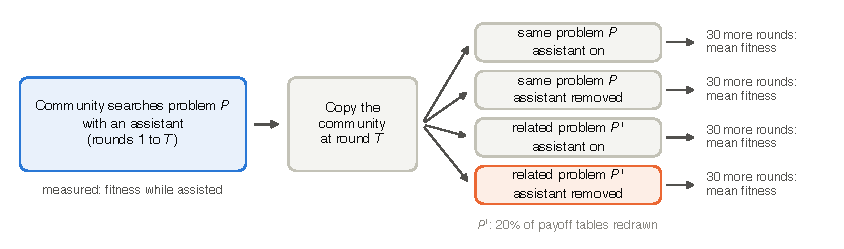
\includegraphics[width=\textwidth]{figures/fig1_probe.pdf}
\caption{The test we add to the model of \citet{fazelpour2026navigating}. After $T$ rounds with an assistant, the community is copied and run for 30 more rounds on the same problem or on a related problem whose payoffs differ for 20\% of the decisions, with the assistant still available or removed. Our main measure is fitness on the related problem with the assistant removed (highlighted).}
\label{fig:probe}
\end{figure}

We report three measures. Each is a percent difference from a community without AI that has the same problem, network, starting approaches and random draws.
\begin{itemize}
\item \emph{Fitness while assisted}: mean fitness over rounds 1 to $T$. This is what an evaluation of the assistant during use would see.
\item \emph{Fitness after}: mean fitness over the 30 rounds after the copy. Our main measure uses the related problem with the assistant removed.
\item \emph{Diversity}: the mean pairwise Hamming distance between teams' approaches, as in \citet{fazelpour2026navigating}.
\end{itemize}
We measure absolute fitness after the change rather than improvement, so that an assistant cannot look good by leaving teams with worse starting points. Unless noted otherwise, we run 1000 simulations per setting and report 95\% confidence intervals from paired differences.

Our implementation reproduces the findings of \citet{fazelpour2026navigating} (Appendix~\ref{app:replication}). NP reduces diversity by 24\% on average (they report 25\%), helps only at high modularity and moderate use, and hurts at high use. TDR outperforms SBP at every use rate when $\rho=1$. SBP helps across modularity levels. One difference is that NP's gains begin at $\rho \approx 0.9$ in our runs, rather than 0.8.

\section{Simulation 1: Help Now, Adapt Later}
\label{sec:sim1}

\subsection{Experimental Design}

We compare NP, TDR and SBP at modularity $\rho \in \{0.6, 0.8, 1\}$ and AI use rates of 0.25, 0.5 and 0.75, with the test applied after $T = 10$, 30, 60 and 100 rounds. To see what drives the differences, we then add three designs at $\rho \in \{0.8, 0.9, 1\}$: PCC, and two variants of TDR meant to reduce homogenization. TDR-25\% samples from the top 25\% of teams instead of the top 10\%. TDR-inverse favors modules that few teams use.\footnote{TDR-inverse draws a team from the top 10\% with probability proportional to one over the number of teams already using its computational module. We also tested variants of SBP that pick at random, or pick the most unusual change, among the few best changes. They behave like SBP, because SBP hardly reduces diversity in the first place (Appendix~\ref{app:sim1}).}

\subsection{Results}

\paragraph{In-use help does not predict what an assistant leaves behind.} Figure~\ref{fig:sim1} plots each design's fitness while assisted against its fitness on the related problem with the assistant removed, after 30 rounds of assistance. At $\rho=1$ and AI use 0.5, NP raises fitness while assisted by 23\% but leaves the community 2\% worse off than a community that never had AI once the problem changes (95\% CI $-4.5$ to $-0.1$). SBP raises fitness while assisted by 18\% and leaves the community 4\% better off afterwards (2.4 to 6.1). An evaluation based on in-use help would rank NP above SBP; an evaluation based on what the community can do after the problem changes would rank it below. Such reversals occur in 14 settings at a strict threshold (Bonferroni-corrected $p < 4.4\times10^{-5}$), all between NP and an SBP-type design at $\rho=1$.

\begin{figure}[t]
\centering
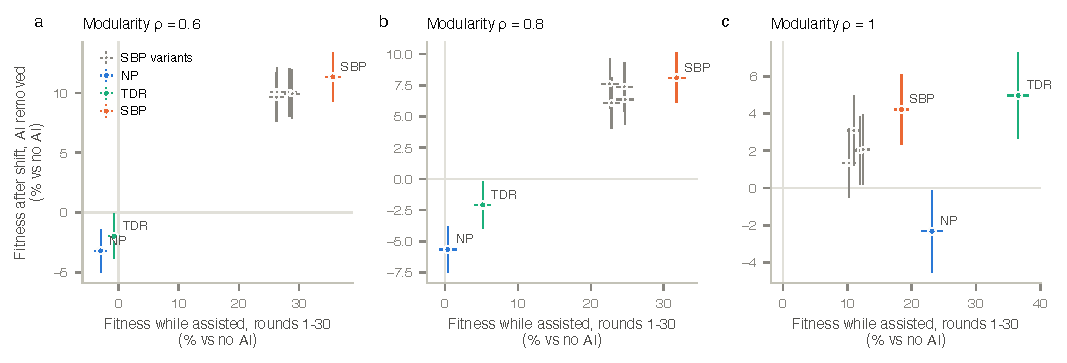
\includegraphics[width=\textwidth]{figures/fig2_help_now_after.pdf}
\caption{Fitness while assisted (rounds 1 to 30, x axis) against fitness over 30 rounds on the related problem with the assistant removed (y axis), each as a percent difference from a community without AI. AI use 0.5; 95\% CIs from 1000 paired simulations. Grey points are SBP variants that pick at random, or pick the most unusual change, among the best few changes.}
\label{fig:sim1}
\end{figure}

\paragraph{The cost comes from handing over whole solutions.} PCC is the most helpful design while in use at every modularity level we tested, up to 44\% at $\rho=1$. But at $\rho=1$ it keeps little of that advantage once the problem changes: 5\% (Figure~\ref{fig:mechanism}b). Compared with staying on the same problem, the change costs PCC 12.6 percentage points and SBP 3.8. The two TDR variants add 1 to 2 points after the change and leave the pattern unchanged. What separates the designs is not how they choose what to recommend but whether they hand over a whole module copied from another team. Every such design halves the community's diversity within about 10 rounds at $\rho=1$ (Figure~\ref{fig:mechanism}a).

\begin{figure}[t]
\centering
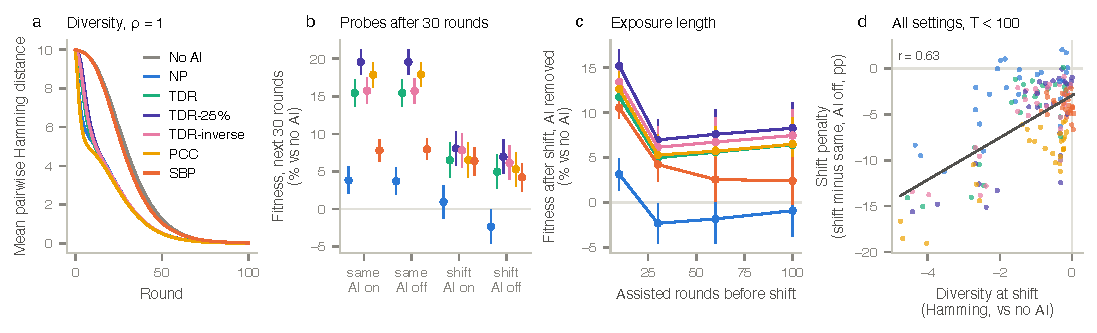
\includegraphics[width=\textwidth]{figures/fig3_mechanism.pdf}
\caption{(a) Diversity over rounds at $\rho=1$, AI use 0.5. (b) Fitness over the 30 rounds after 30 assisted rounds, in the four conditions of Figure~\ref{fig:probe}. (c) Fitness on the related problem with the assistant removed, by the number of assisted rounds before the change. (d) Each point is one design, modularity, use rate and $T<100$: the cost of the change (fitness on the related problem minus fitness on the same problem, both with the assistant removed, in percentage points) against diversity at the change relative to no AI. Line: least squares fit. 1000 simulations per setting.}
\label{fig:mechanism}
\end{figure}

\paragraph{The cost tracks lost diversity.} Across all designs and settings, the cost of the change correlates with how much diversity the assistant removed by the time of the change: $r = 0.46$ across the settings in Figure~\ref{fig:sim1} and $r = 0.63$ across those in Figure~\ref{fig:mechanism}d. Teams in a homogeneous community start the new problem from the same place, and they have no different approaches to learn from.

\paragraph{The cost appears early.} The advantage that remains after the change shrinks over the first 30 rounds of assistance and stays about level afterwards (Figure~\ref{fig:mechanism}c). Since all communities eventually converge, even without AI \citep{fazelpour2026navigating}, the difference is in how quickly a community narrows, not in where it ends up.

\paragraph{Robustness.} The pattern holds with a denser network, a larger change, and a smoother landscape (Table~\ref{tab:robust}; Appendix Figure~\ref{fig:robust}). With 50\% of the payoffs redrawn, PCC goes from 44\% while assisted to $-1$\% afterwards, and SBP is the only design that still leaves the community better off than no AI.

\begin{table}[t]
\centering
\small
\caption{Robustness of Simulation 1 at $\rho=1$, AI use 0.5, $T=30$. Fitness while assisted and on the related problem with the assistant removed, percent difference from no AI. Reversals: pairs of designs and settings where one design is better while assisted and the other is better afterwards, both at Bonferroni-corrected $p<6.2\times10^{-5}$. $r$: correlation between the cost of the change and diversity lost.}
\label{tab:robust}
\begin{tabular}{lccccc}
\toprule
Setting & PCC while / after & SBP while / after & NP while / after & Reversals & $r$ \\
\midrule
Main (edge 0.05, 20\% change, $K=9$) & 43.6 / 5.3 & 18.4 / 4.2 & 23.2 / $-$2.3 & 6 & 0.63 \\
Denser network (edge 0.1) & 37.5 / 6.0 & 15.4 / 5.2 & 17.6 / $-$1.1 & 8 & 0.52 \\
Larger change (50\%) & 43.6 / $-$1.3 & 18.4 / 1.8 & 23.2 / $-$2.8 & 14 & 0.48 \\
Smoother landscape ($K=5$) & 38.1 / 1.3 & 22.7 / 4.8 & 22.2 / $-$2.6 & 16 & 0.49 \\
\bottomrule
\end{tabular}
\end{table}

\section{Simulation 2: Learning When to Help}
\label{sec:sim2}

Simulation 1 suggests that full answers cost adaptability and nudges do not, but full answers help much more in the moment. Can an assistant get the benefits of both? And does it need a reward that looks beyond the moment?

\subsection{Experimental Design}

We train an assistant that, each time a team asks, chooses one of three actions: give a full answer (as PCC), give a nudge (as SBP), or step back. The choice depends on six features: the round, the community's diversity, the asking team's rank, the gain the full answer and the nudge would each bring, and how many teams already use the module the full answer would give.\footnote{The policy is a softmax over a linear score of the features, with about 15 parameters, trained with an evolution strategy. We train on 800 problems and test on 200 others at $\rho \in \{0.8, 0.9, 1\}$, AI use 0.5 and $T=30$. We also test on a 50\% change and on AI use 0.75, neither of which the policy saw in training.} We train it with three rewards:
\begin{itemize}
\item $R_{\text{now}}$: mean fitness while assisted, the immediate reward;
\item $R_{\text{long}}$: $R_{\text{now}}$ plus mean fitness over 30 more rounds with the assistant still available;
\item $R_{\text{adapt}}$: $R_{\text{now}}$ plus mean fitness over 30 rounds on the related problem with the assistant removed.
\end{itemize}
If looking only at the moment were the problem, $R_{\text{adapt}}$ should produce a different assistant. We compare the learned policies with fixed rules: always a full answer, always a nudge, mixes of the two, schedules that give full answers first and nudges later, and \emph{gated} rules that help only when the help would improve the asking team and otherwise step back.

\subsection{Results}

\paragraph{The reward horizon does not matter.} All three rewards produce the same policy, and two independent training runs per reward agree within 2 percentage points. Each policy helps heavily in the first five rounds, nudging first and then giving full answers, and steps back about 85\% of the time afterwards (Appendix Figure~\ref{fig:p2actions}). At $\rho=1$, the policy trained on $R_{\text{now}}$ raises fitness while assisted by 87\% and fitness on the related problem by 27\%; the policy trained on $R_{\text{adapt}}$ gets 86\% and 27\% (Figure~\ref{fig:sim2}).

\paragraph{Stepping back is what matters.} The learned policies outperform every rule that always answers. The best of those rules, 25\% full answers and 75\% nudges, gets 68\% and 24\%. A one-line gated rule, which helps with whichever action gains more and otherwise steps back, gets 85\% and 25\%, close to the learned policies. When an assistant's help would not improve a team, the team spends a round rejecting it. An assistant that steps back in those cases leaves teams to explore, which helps now and keeps more variety for later.

\paragraph{Mixing matters too.} The gated rule that gives only full answers gets 55\% and 9\%; mixing full answers with nudges does much better. Nudges find new improvements, and full answers spread them.

\begin{figure}[t]
\centering
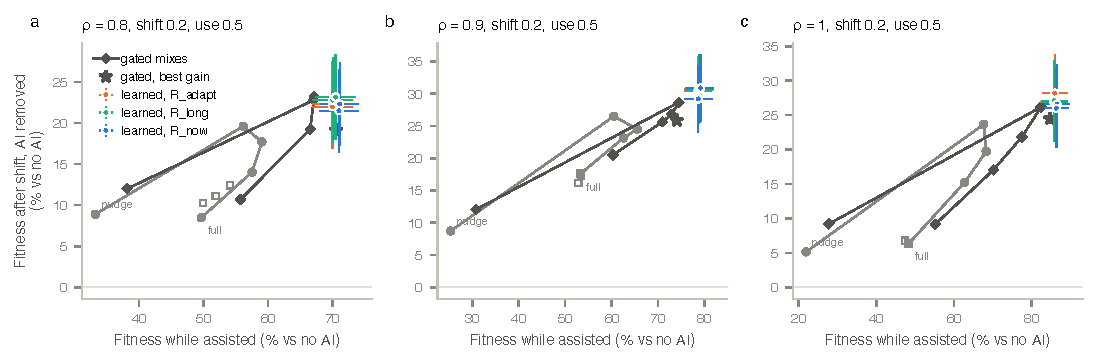
\includegraphics[width=\textwidth]{figures/fig4_learned.pdf}
\caption{Learned policies and fixed rules on 200 held-out problems, AI use 0.5. Grey circles: rules that always answer, from all nudges to all full answers. Squares: full answers first, then nudges. Dark diamonds: gated rules that help only when the help would improve the team and otherwise step back; star: gated rule with whichever action gains more. Coloured points: policies learned with the three rewards, with 95\% CIs.}
\label{fig:sim2}
\end{figure}

These results suggest that the cost found in Simulation 1 is not a matter of reward horizon, at least in this model. An assistant that maximizes immediate help, given the option to step back and both kinds of help, already does well later.

\section{Simulation 3: Help Across a Sequence of Problems}
\label{sec:sim3}

Real communities face one problem after another. We run each community through four problems in a row, 60 rounds each. Each problem redraws 20\% of the previous problem's payoffs, and the assistant stays available throughout. We run 300 simulations per assistant.

Every assistant helps most on the first problem and much less afterwards (Figure~\ref{fig:sim3}). At $\rho=1$, PCC raises fitness while assisted by 28\% on the first problem and by 4\%, $-4$\% and 3\% on the next three, none of which is clearly different from no AI. SBP goes from 13\% to between 3\% and 6\%. The gated rule from Simulation 2 goes from 59\% to 17\%, 6\% and 6\%, and is the only assistant clearly ahead of no AI on every problem. The pattern is similar at $\rho=0.8$.

\begin{figure}[t]
\centering
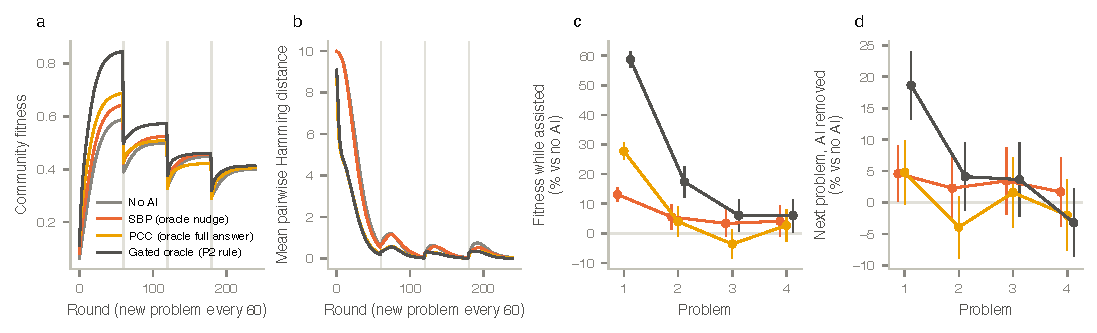
\includegraphics[width=\textwidth]{figures/fig5_sequence.pdf}
\caption{Four problems in a row, 60 rounds each, $\rho=1$, AI use 0.5, 300 simulations per assistant. (a) Fitness and (b) diversity over rounds; vertical lines mark a new problem. (c) Mean fitness while assisted in each problem and (d) mean fitness over 30 rounds on the next problem with the assistant removed, as percent differences from no AI with 95\% CIs.}
\label{fig:sim3}
\end{figure}

The reason is that every community converges during the first problem. PCC works by recombining what other teams already have, so once every team holds the same module it has nothing left to offer. Help that brings in something new, like SBP's single changes, also runs out once the community sits at a shared local optimum. This sets up the question for language model assistants. An assistant whose knowledge comes from the community it advises behaves like PCC.

\section{Language Model Assistants That Learn from Users}
\label{sec:llm}

The assistants so far know the true payoffs. A deployed language model does not. It learns what helps from feedback on its answers, and the feedback it gets depends on the people it has already helped. We now let a language model play the assistant and keep learning from the community.

\subsection{Setup}

The assistant is Qwen3-4B-Instruct \citep{yang2025qwen3} with low-rank adapters \citep[LoRA;][]{hu2022lora}. When a team asks, the model sees the team's 20 decisions as digits and replies with ten digits for the computational module. It never sees the payoffs. After each round, we update it with GRPO: for each team that asked, we sample 8 answers, score each one, show the team one of them, and increase the probability of answers that scored better than the average of their group.\footnote{Training details and the exact prompts are in Appendix~\ref{app:llm}.} Each community goes through four problems in a row, as in Simulation 3, at $\rho \in \{1, 0.8\}$ and AI use 0.5.

To see what a trained assistant leaves behind, we freeze the model after each problem and run it as the assistant for 100 to 200 fresh communities on the same problem, followed by the test of Figure~\ref{fig:probe}. The oracle designs, no AI and the untrained model serve the same communities. This gives a precise estimate for each trained model. Since each training run sees one problem sequence, we treat the training run as the unit of analysis and report confidence intervals over training runs.

\subsection{Learning Only from Its Own Help}

We first train the model on the gain its answer brings to the asking team, on the same gain with a KL penalty toward the untrained model, and on the same gain with the option to step back (returning the team's current choices unchanged, in which case the team explores). With every signal, the model collapses during the first problem. In the second half of the problem, 83\% to 100\% of teams that ask get the same answer, and the 8 sampled answers for a single team are nearly identical (1.0 to 1.6 distinct answers), which leaves GRPO no signal to learn from. Only the KL penalty keeps the answers varied: 2.2 to 4.1 distinct answers out of 8 ($p = 0.007$ against the gain alone at $\rho=0.8$; $p = 0.07$ at $\rho=1$; 6 training runs each). The option to step back does not help; the model learns to step back almost always, or collapses onto one answer.

In this setting the collapse matters little for the community. Run on fresh communities, the collapsed model gives 14 distinct answers to about 54{,}000 requests, but those answers rarely help, so teams do not adopt them. It is about as good as no AI ($-2$\%, 95\% CI $-15$ to 11), and the community's diversity drops only slightly (4.1 against 4.7 without AI). A model that gives everyone the same answer makes a community alike only if its answer is taken up.

\subsection{Seeing What Works for Others and Learning from User Feedback}

A deployed assistant knows what works for others. We add the three best distinct approaches in the community, with their scores, to the prompt. We train the model with the two kinds of feedback developers collect from users:
\begin{itemize}
\item \emph{Thumbs up or down}: the team tries the answer and gives a thumbs up if it improved their score.
\item \emph{Pick one of two}: the team sees two answers and picks the one that is better for them. When both are equally helpful, or equally useless, they pick at random, but they always prefer a well-formed answer to a malformed one.\footnote{An earlier version picked at random between a malformed and a useless well-formed answer. Without a KL penalty, one training run per modularity then drifted into free text. Requiring the simulated team to prefer well-formed answers removed the drift but not the collapse.}
\end{itemize}
We also train on the scalar gain, as before, and run thumbs and pick-one-of-two both with and without a KL penalty. We use 6 training runs per variant at both modularity levels, and 12 training runs for thumbs and pick-one-of-two at $\rho=1$.

\paragraph{With context, the model learns to copy the best approach for everyone.} Within a few rounds nearly every team gets the same answer, and the community converges almost as fast as with PCC. At $\rho=1$, after 10 rounds about 5 to 8 distinct computational modules remain, against 47 without AI, 32 with SBP and 1.2 with PCC. Pick-one-of-two collapses completely, giving one answer to 98\% to 100\% of teams. Thumbs keeps somewhat more variety, 0.73 more distinct answers out of 8 (95\% CI 0.44 to 1.01; 12 training runs). Unlike the model without context, this model keeps pointing each community to what currently works best in it, so its answers help fresh communities and get adopted.

\paragraph{It helps as much as a nudge now and leaves the community worse placed later.} Figure~\ref{fig:llm_eval} shows the frozen models after the first problem, run on fresh communities. At $\rho=1$, the models trained on thumbs and on pick-one-of-two raise fitness while assisted by 21\% (95\% CI 11 to 31; 12 training runs each), about the same as SBP (difference 3 points, CI $-6$ to 12). But on the related problem with the assistant removed, they leave the community 11 percentage points behind SBP (95\% CI $-17$ to $-6$, $p=0.001$), and they halve its diversity (2.5, against 4.4 with SBP and 4.8 without AI). The other variants, with a KL penalty or trained on the scalar gain, look the same. This is the pattern of Simulation 1, now produced by a learned assistant: help that looks like a nudge in the moment, with the cost of a full answer afterwards.

\begin{figure}[t]
\centering
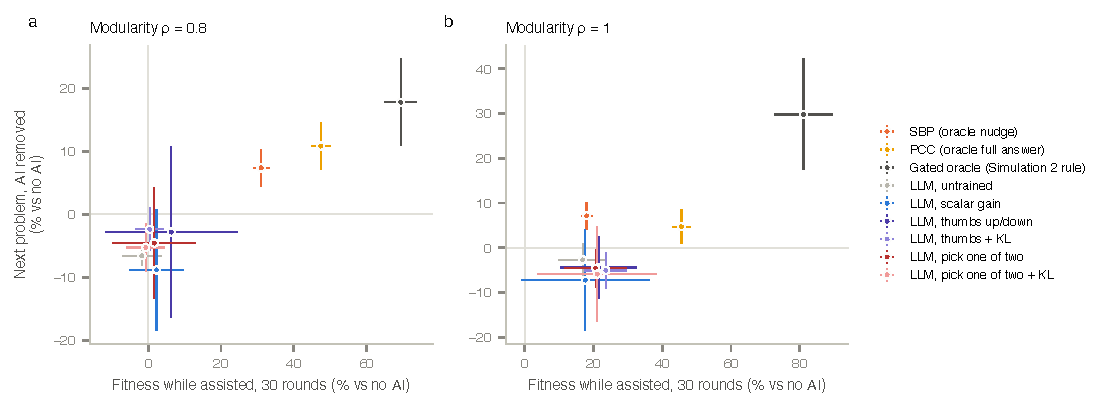
\includegraphics[width=\textwidth]{figures/fig6_llm_frozen.pdf}
\caption{Language model assistants with the community's best approaches in the prompt, frozen after the first problem and run on 100 fresh communities per training run. Axes as in Figure~\ref{fig:sim1}. Oracle designs and the untrained model serve the same communities. 95\% CIs over training runs: 12 for the oracles, the untrained model, thumbs and pick-one-of-two at $\rho=1$, and 6 otherwise.}
\label{fig:llm_eval}
\end{figure}

\paragraph{The cost persists over training, and user feedback does not remove it.} Figure~\ref{fig:llm_gap} follows the gap to SBP across the four checkpoints with 12 training runs. While in use, both models stay level with SBP throughout. On the related problem with the assistant removed, the model trained on pick-one-of-two stays 8 to 12 percentage points behind SBP at every checkpoint (all $p < 0.05$). The model trained on thumbs is 11, 8, 2 and 5 points behind ($p = 0.008$, 0.053, 0.60 and 0.031). Thumbs does slightly better than pick-one-of-two afterwards, by 2.5 points on average, which is not significant. The untrained model given the same context is already 10 points behind SBP after the first problem, so most of the cost comes from what the assistant is shown rather than from how it is trained. At $\rho=0.8$, where the best computational module depends on a team's other decisions, the language model helps little in the moment (24 to 37 points below SBP) and is 6 to 14 points behind SBP afterwards.

\begin{figure}[t]
\centering
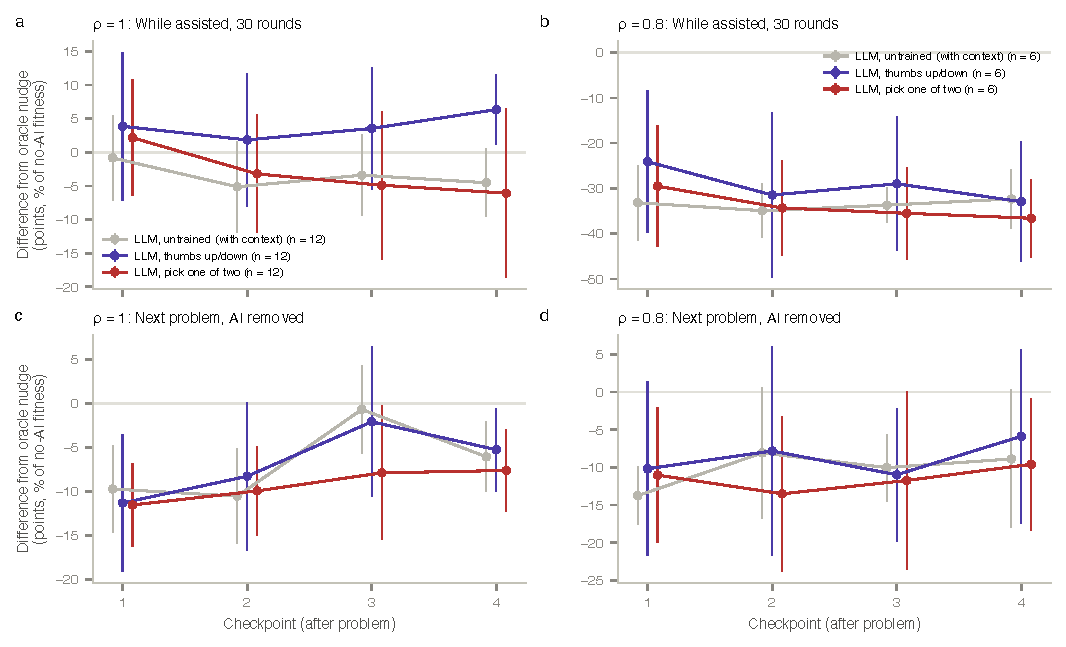
\includegraphics[width=\textwidth]{figures/fig7_gap_over_training.pdf}
\caption{Difference from SBP, in percentage points of no-AI fitness, for language model assistants frozen after each of the four problems. Top: fitness while assisted. Bottom: fitness on the related problem with the assistant removed. Each checkpoint is run on 100 fresh communities per training run; 95\% CIs over training runs (12 at $\rho=1$, 6 at $\rho=0.8$).}
\label{fig:llm_gap}
\end{figure}

\subsection{A Second Model Family}

\pending{Gemma 3 4B \citep{gemma2025gemma3}: same design as the 12-run Qwen result (context, thumbs and pick-one-of-two, $\rho=1$). Results to be added when the runs finish.}

\section{Discussion}
\label{sec:discussion}

\subsection{Evaluating Assistance by What It Leaves Behind}

Our first result is about measurement. Two assistants that look equally helpful during use can leave a community very differently able to deal with the next problem, and in some settings in-use help ranks assistants in the wrong order. An evaluation that looks only at the moment, whether a benchmark, a user study or the feedback used for training, cannot see this. The test we use is simple: copy the community, change the problem, remove the assistant, and measure. Similar tests are possible with people, as in studies that measure performance after AI help is removed \citep{bastani2025generative,kumar2025human}. Our results suggest running them with groups, where homogenization shows up, and after a change in the task.

\subsection{What Kind of Help to Give}

Our second result is about design. The cost comes from handing over whole solutions that other people already use, and it is avoided by small changes and by stepping back. A longer reward horizon does not change what a learned assistant does; the option to step back does. This fits with work on assistants that leave decisions to people \citep{myers2024learning} and with the finding that tutors with guardrails protect learning \citep{bastani2025generative}. It also points to a limit of randomization as a fix for homogenization \citep{jain2024scarce}. In our model, randomizing which full answer to give barely helps, because the cost comes from the size of the change, not from which answer is chosen.

\subsection{What User Feedback Can See}

Our third result is about training. A language model that sees what works for others and learns from user feedback ends up copying the best approach for everyone. Each team that adopts the copied approach is better off, so feedback rewards it. The cost appears only later, only when the problem changes, and only for the community as a whole, so no single thumbs up or choice between two answers can reflect it. A KL penalty keeps the model's own answers varied, but it does not keep the community varied. And most of the cost is already present in an untrained model shown the same context. What an assistant is shown about others may matter as much as how it is trained.

\subsection{Assumptions, Limitations, and Future Directions}

Like any model, ours relies on idealizing assumptions. We note those that matter most for our conclusions.

Teams in our model evaluate every recommendation perfectly and adopt only improvements. In practice, people often cannot tell whether a suggestion helps, especially in the areas where they rely on AI \citep{fazelpour2026navigating}. Rejected recommendations cost only a round, while in practice an adopted bad recommendation can cost much more. Both points suggest that our model understates the cost of full answers.

Teams do not lose skill in our model: assistance changes where they are in the space of approaches, not how well they search. Reliance on AI may also change what people can do on their own \citep{bastani2025generative}, which our model does not capture. Our results show a cost that arises even without any loss of skill.

All communities in the model eventually converge, even without AI, so our results concern how fast a community narrows. Turnover, new members or changing goals would keep communities more varied and could change the size of the effects.

The change between problems is random and of fixed size. Larger changes make the cost larger (Table~\ref{tab:robust}). We did not study changes that target what the community has converged on.

The language model study uses small models, a simple prompt and 6 to 12 training runs per variant. \pending{Replication across model families, Section 7.4.} Larger models, richer tasks and other training methods may behave differently.

Finally, the members of our communities are simple rules, not people. We chose this on purpose, since simulations of people with language models can be homogeneous on their own. Experiments with groups of people, in the style of \citet{kumar2025human}, are the natural next step.

\section{Conclusion}

How much an assistant helps while in use is the standard way to judge and train it. In a simple model of collective search, we find that this can give the wrong answer about what an assistant leaves behind. Assistants that hand over whole solutions help most in the moment and leave communities less able to adapt; assistants that nudge, or step back when they have nothing to add, do not. A language model that learns from user feedback and sees what works for others drifts toward the first kind. Measuring what assistance leaves behind, and not only what it does in the moment, is a first step toward assistants that help without narrowing the communities they serve.

\bibliographystyle{plainnat}
\bibliography{refs}

\appendix

\section{Replication of Fazelpour et al.}
\label{app:replication}

Figure~\ref{fig:replication} reproduces the main figures of \citet{fazelpour2026navigating}: the difference from no AI in final fitness, early fitness and diversity for NP, TDR and SBP across modularity and AI use rates, with $N=20$, $M=10$, $K=9$, $H=10$, $p_{\text{social}}=0.1$ and 1000 simulations per cell. Three choices are not specified in their paper: the network's edge probability (we use 0.05), the fitness transform (we use the exponent 8 of \citet{lazer2007network}; it does not affect dynamics), and the update order (we update all teams at once, each acting on the state at the start of the round).

\begin{figure}[h]
\centering
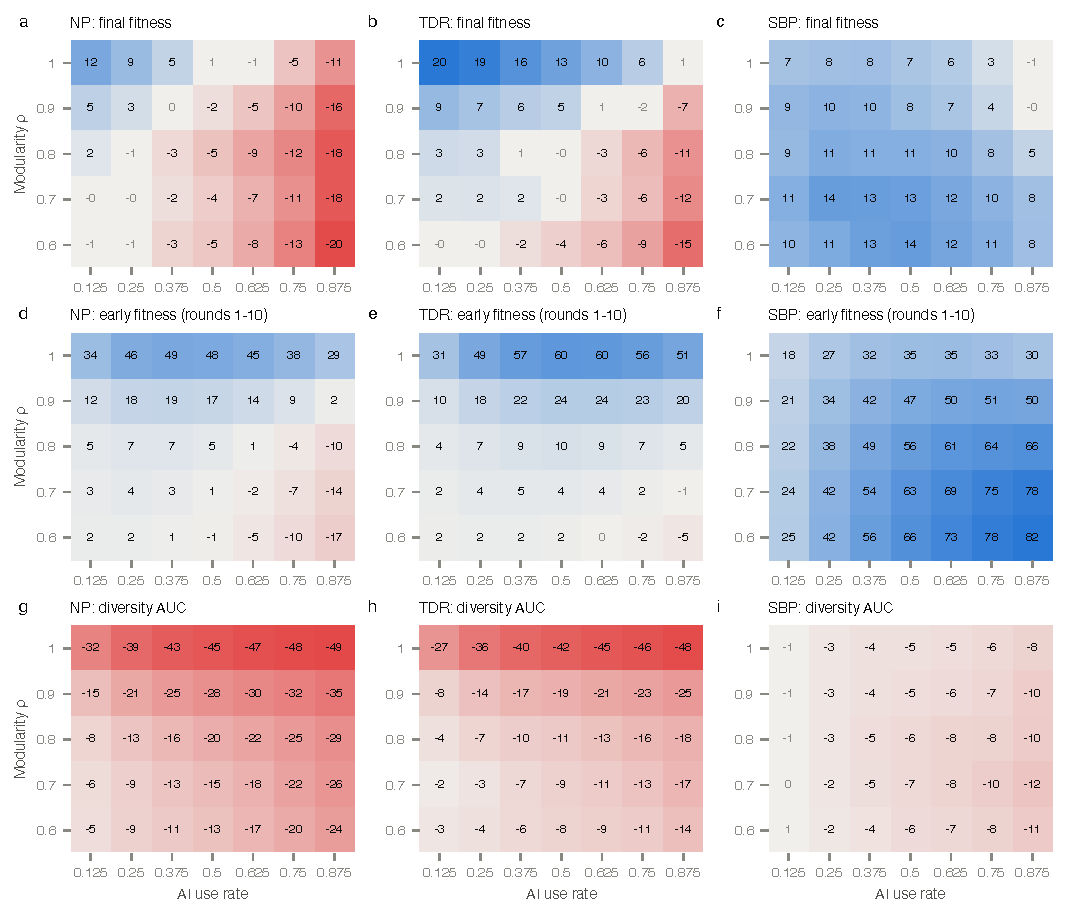
\includegraphics[width=\textwidth]{figures/figA1_replication.pdf}
\caption{Replication. Percent difference from no AI in fitness at round 100 (top), mean fitness in rounds 1 to 10 (middle) and the area under the diversity curve (bottom). Grey cells: paired $t$-test $p \geq 0.05$. 1000 simulations per cell.}
\label{fig:replication}
\end{figure}

\section{Additional Results for Simulations 1 and 2}
\label{app:sim1}

Variants of SBP that pick at random, or pick the change that moves the team furthest from the others, among the 3 best or all improving changes, behave like SBP (Figure~\ref{fig:sim1}, grey points). Figure~\ref{fig:robust} shows the robustness checks summarized in Table~\ref{tab:robust}. Figure~\ref{fig:p2actions} shows what the learned policies of Simulation 2 do over the assisted rounds.

\begin{figure}[h]
\centering
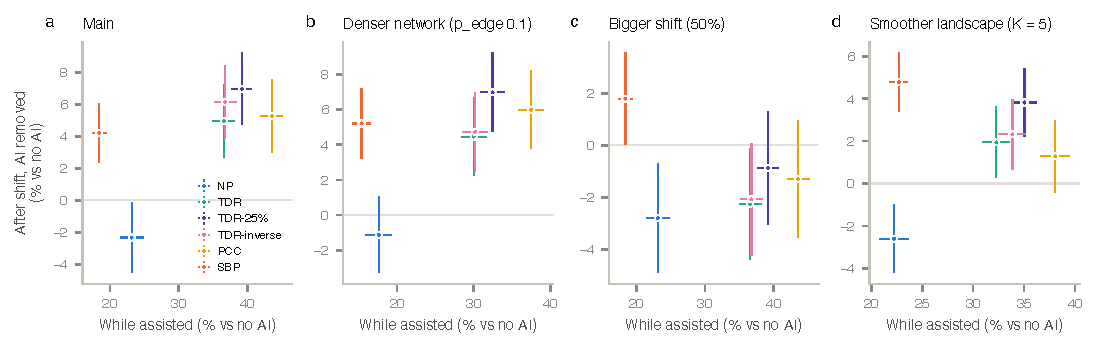
\includegraphics[width=\textwidth]{figures/figA2_robustness.pdf}
\caption{Robustness of Simulation 1 at $\rho=1$, AI use 0.5, $T=30$: the main setting, a denser network, a larger change and a smoother landscape. Axes as in Figure~\ref{fig:sim1}.}
\label{fig:robust}
\end{figure}

\begin{figure}[h]
\centering
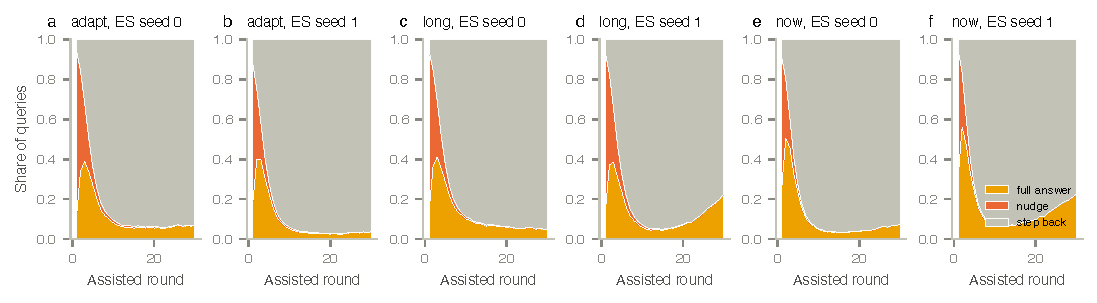
\includegraphics[width=\textwidth]{figures/figA3_policy_actions.pdf}
\caption{Share of requests answered with a full answer, a nudge, or a step back, by assisted round, for the policies learned with the three rewards ($\rho=1$, AI use 0.5).}
\label{fig:p2actions}
\end{figure}

\section{Language Model Details}
\label{app:llm}

\paragraph{Prompt.} The system message is ``You help research teams improve their approach.'' The user message is: ``A team's approach is 20 yes/no choices, written as digits (1 = yes). Choices 1-10 (you can change these): [ten digits]. Choices 11-20 (fixed): [ten digits]. Recommend values for choices 1-10. Reply with exactly ten digits and nothing else.'' With context, the message starts with ``Approaches the best-scoring teams use right now (choices 1-10 | choices 11-20, score):'' followed by the three best distinct approaches in the community. With the step-back option, it ends with ``If no change would help, repeat the current values and the team will explore on its own.'' We take the first run of ten binary digits in the reply as the answer; replies without one are treated as no recommendation.

\paragraph{Training.} LoRA with rank 16 on the attention and feed-forward projections of the language model, learning rate $5\times10^{-5}$, one GRPO step per round with 8 samples per request at temperature 1, advantages normalized within each group of 8. The KL penalty, when used, has weight 0.05 toward the untrained model. The scalar reward is the gain in the asking team's fitness (zero if the answer does not improve it). Each training run covers four problems of 60 rounds; we save the adapter after each problem.

\paragraph{Frozen evaluation.} Each saved adapter is run with vLLM at temperature 1 for 100 (Section~\ref{sec:llm}, context) or 200 (no context) fresh communities on the problem it last trained on, for 30 assisted rounds, followed by the four conditions of Figure~\ref{fig:probe}.

\paragraph{Additional figures.} Figure~\ref{fig:llm_dyn} shows training dynamics for the runs with context at $\rho=1$.

\begin{figure}[h]
\centering
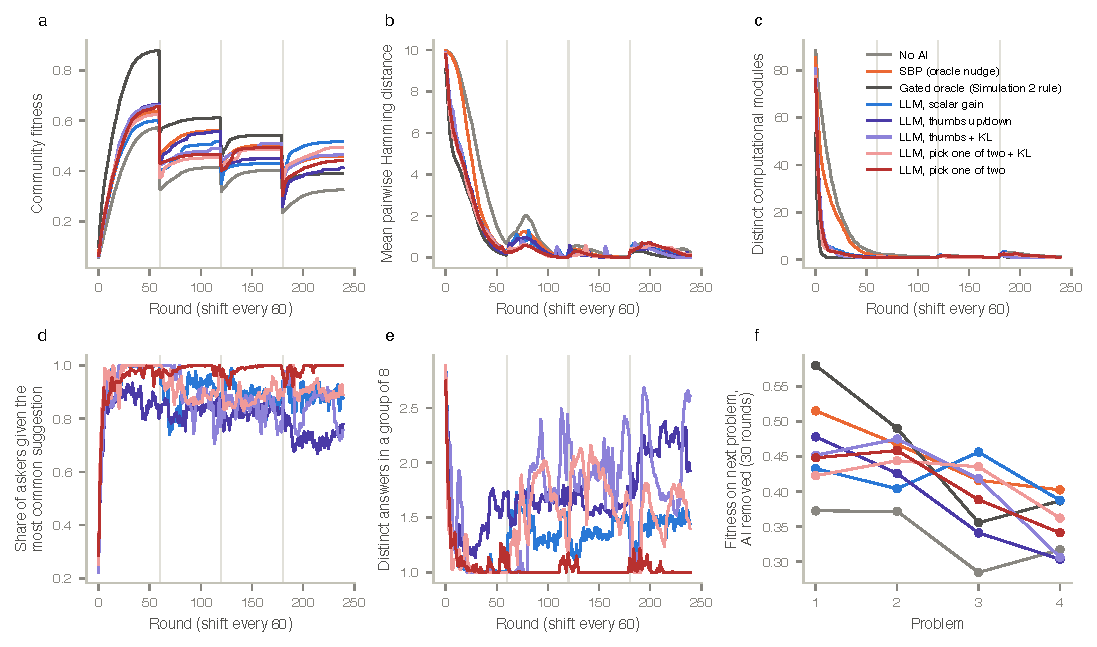
\includegraphics[width=\textwidth]{figures/figA4_llm_training.pdf}
\caption{Training runs with the community's best approaches in the prompt, $\rho=1$. (a) Community fitness, (b) diversity and (c) distinct computational modules over rounds, with oracle baselines on the same problems. (d) Share of asking teams given the most common answer. (e) Distinct answers among the 8 sampled per request. (f) Fitness on the next problem with the assistant removed. Means over training runs.}
\label{fig:llm_dyn}
\end{figure}

\end{document}
